%Plantilla anteproyecto
%Última modificación: 21 de mayo de 2010
\documentclass[12pt,oneside,a4paper]{article}
\usepackage[spanish]{babel}
\usepackage[utf8]{inputenc}
\usepackage{graphicx}
\usepackage{float}
\usepackage{amsmath}
\usepackage{amssymb}
\usepackage{color}
\usepackage{colortbl}
\usepackage{subfigure}
\usepackage{url}
\usepackage[all]{xy}
\linespread{1}
\setlength{\parskip}{1\baselineskip}
\parindent 1cm
\sloppy


%Opciones que debes descomentar mientras estemos revisando el anteproyecto
%\usepackage{lineno}
%\linenumbers
\usepackage[pagebackref=true,breaklinks=true,letterpaper=true,colorlinks,bookmarks=true]{hyperref}


%lista de palabras que Latex no parte bien
\hyphenation{pa-la-bras lis-ta}

\begin{document}

\thispagestyle{empty}

\begin{center}


Departamento de Teoría de la Señal y Comunicaciones\\
Escuela Politécnica Superior\\
Universidad de Alcalá\\

\vspace{1cm}


\includegraphics[width=4cm]{figuras/logo-uah.eps}

\textbf{ANTEPROYECTO}

\vspace{1cm}

\begin{large}\textbf{\textit{Sistema de adaptación inteligente de la velocidad para vehículos basado en inteligencia artificial y visión por computador}}\end{large}

\vfill

Enero - 2021

\end{center}

\begin{flushright}
\textit{Autor - \textbf{Sergio Sastre Arrojo}} \\
\textit{Director - \textbf{Roberto Javier López Sastre}}
\end{flushright}

\newpage
\section{Introducción}

En los últimos años, con la aparición de los sistemas de adaptación inteligente de la velocidad (ISA), se han evitado muchas desgracias afortunadamente. No obstante, la tecnología actual viene con una serie de limitaciones que se podrían mejorar. Por ejemplo: la mayoría de estos sistemas utilizan GPS, lo cual es muy eficiente para su propósito, pero en determinadas ocasiones (núcleos urbanos, distinción de carriles en una autovía con una carretera de servicio) pueden desembocar en situaciones de gran peligro.

¿Pero qué es un sistema ISA? ISA son las siglas de Intelligent Speed Adaptation, y como su propio nombre indica, es un sistema para adaptar la velocidad según diversos factores como: adaptación por proximidad con otros vehículos u objetos, o por GPS como hemos mencionado anteriormente.

Es por ello que aquí presentamos una solución ante esos problemas: \[ISA^{2}\]

Con este nuevo sistema queremos adaptar la velocidad del vehículo en base a la situación del tráfico en cada momento, la situación que el vehículo observa mediante una cámara frontal. Una primera aproximación a este problema ya ha sido implementada \cite{isa2}, y el principal objetivo de este TFG es mejorar ese sistema para hacerlo más preciso y práctico.


\section{Objetivos y campos de aplicación}

Como ya hemos dicho, el objetivo principal de este proyecto es optimizar la primera versión del sistema $ISA^{2}$.

Para ello, realizaremos una repetición de los experimentos detallados en \cite{isa2}, para comprobar que las nuevas mejoras funciona correctamente y de forma más eficiente que el anterior.

En cuanto a los campos de aplicación, cabrían destacar los siguientes:
\begin{enumerate}
 \item Este proyecto será aplicable a cualquier campo relacionado con el automovilismo, para ayudar a mejorar la seguridad vial actual y para facilitar la lectura de la vía durante la conducción. En esencia, todo lo anterior se puede resumir en lo siguiente:
 \begin{enumerate}
 	\item Implementación de soluciones de adaptación de velocidad inteligente.
 	\item Implementación de sistema de detección de situaciones peligrosas en función de la velocidad.
 	\item Desarrollo de nuevas ayudas a la conducción más inteligentes.
 \end{enumerate}
\end{enumerate}



\section{Descripción del trabajo}

A continuación vamos a pasar a explicar las fases sobre las que se va a desarrollar el proyecto. Para ello nos ayudaremos de un diagrama de bloques.

\begin{figure}[h]
  \centering
  \includegraphics[width=16cm]{figuras/Diagrama_Bloques.eps}
  \caption{Diagrama de bloques}
  \label{fig:diagrama_bloques}
\end{figure}


Como se puede ver en la Figura \ref{fig:diagrama_bloques}, comenzaremos con una exploración de nuevos modelos de predicción de segmentación semántica. La idea es integrar en el sistema $ISA^2$ los últimos modelos de segmentación semántica y de predicción de la misma, que definen el estado del arte. 

\begin{figure}[H]
  \centering
  \includegraphics[width=4cm]{figuras/Figura_Esquema_ISA2_Version_1_SegSem.eps}
  \caption{$ISA^2$ Versión 1}
  \label{fig:isa_v1}
\end{figure}

Como se muestra la Figura \ref{fig:isa_v1}, el algoritmo que se utiliza en \cite{isa2} se basa en una CNN (Convolutional Neural Network) desde la que le pasamos como entrada una imagen en diferentes escalas. Para esa versión se utilizó el modelo DeepLab \cite{deeplab} como framework para hacer uso del algoritmo de segmentación semántica, teniendo como base una CNN (en este caso, ResNet-101). Este proceso queremos mejorarlo en esta nueva versión: utilizando otros frameworks u otros modelos de CNN para segmentación semántica. 

También exploraremos nuevas soluciones para la predicción de la segmentación semántica, como \cite{segmpred}. De este modo añadiremos al sistema $ISA^2$ la posibilidad de anticipar la predicción de la velocidad.

Una vez exploradas estas técnicas, se procederá a la implementación e integración de las mismas, en el modelo $ISA^2$, para poder evaluar su eficacia en cuanto a estimación de la velocidad. 

Una vez la implementación esté finalizada, procederemos a la evaluación experimental. Para ello emplearemos la base de datos proporcionada en \cite{isa2}. Aquí realizaremos una comparativa exhaustiva con las anteriores soluciones, para validar la efectividad de los nuevos modelos propuestos.


\section{Fases de desarrollo}

Teniendo en cuenta el apartado anterior, vamos a pasar a explicar de forma más detallada las diferentes fases del proyecto que antes hemos nombrado y descrito:

\begin{enumerate}
 \item Exploración de nuevos modelos y técnicas de predicción de segmentación semántica (2 semanas)
 \item Integración de las mismas en el sistema (1 mes y 2 semanas)
 \item Realización de experimentos sobre el nuevo sistema para comprobar su funcionamiento (1 mes y 2 semanas)
 \item Realización de memoria en LaTex (4 meses)
 \item Conclusiones (2 semanas)
 %Enumera, de forma esquemática los pasos en los que se traducen la descripción del trabajo que has escrito arriba. Tal y como venía en la plantilla que te pasé.
\end{enumerate}

\section{Medios disponibles}

Dispondremos de las siguientes herramientas:

\begin{enumerate}
	\item Estación de trabajo con GPU (NVIDIA 1080 TI) para la realización de experimentos con sistema operativo Ubuntu.
	\item Acceso a diferentes librerías de Deep Learning:
	\begin{itemize}
	\item PyTorch
	\item TensorFlow 
	\item Caffe
	\end{itemize}
	\item Acceso a la base de datos $ISA^2$ utilizada en la primera versión \cite{isa2} a través del siguiente enlace: \url{http://agamenon.tsc.uah.es/Personales/rlopez/data/isa2/index.html}.
\end{enumerate}

 






%Bibliografía
\bibliographystyle{plain}
\bibliography{bibliografia-anteproyecto}


\end{document}
